\section{Az útvonaltervező felépítése és működése}

Az első pontban kitértem az összes olyan elméleti részre, ami az útvonaltervező működésének megértéséhez szükséges. Ez a pont egy átvezetés lesz az elmélet és az elkészített C++ implementáció között. Bemutatom az általam elkészített modul tervét és a hozzá tartozó implementációk egy részét, amik szükségesek a teljes felépítés megismeréséhez.

\subsection{A \emph{Waypoint Module} kompozit}

Az általam készített \emph{Waypoint Module} tartalmazza a RC-k generálásához, tárolásához és lekérdezéséhez szükséges logikát. Ezen felül tartalmaz statikus segédfüggvényeket is, amik főleg az RC-k kiszámításánál szükségesek. Minden osztály és (egyéb forráskód is, ahol lehetséges) egy \emph{header} és egy vagy több \emph{source file-ra} van felosztva. Az osztályok és azok metódusai (vagy a statikus függvények definíciói) a megfelelő {\fontfamily{cmtt}\selectfont *.hpp} \emph{file-ban}, míg az implementációk a hozzá tartozó {\fontfamily{cmtt}\selectfont *.cpp} \emph{file-ban}. \emph{Template-et} használó osztályok vagy metódusok esetén az implementáció a {\fontfamily{cmtt}\selectfont *.inl} \emph{file-ban} történik. Erre azért van szükség, mert \emph{template-tel} rendelkező osztályokat vagy metódusokat nem lehet {\fontfamily{cmtt}\selectfont *.cpp} \emph{file-ban} implementálni. Ez azért van, mert a C++ \emph{template-ek} fordítási időben keletkeznek, tehát a \emph{compiler-nek} a teljes definícióra szüksége van, hogy példányosítani tudja őket más fordítási egységekben. Kivétel ez alól a {\fontfamily{cmtt}\selectfont CWaypointModuleParams} osztály, melynek csak \emph{getter} és \emph{setter} függvényei vannak a belső értékekre. Mivel ezek implementációja triviális, ezért a megfelelő {\fontfamily{cmtt}\selectfont .hpp} állományban vannak {\fontfamily{cmtt}\selectfont inline} előtaggal ellátva. Ez azt eredményezi, hogy a fordító minden függvényhívásnál kicseréli a hívást a bennelévő implementációval. Ennek segítségével gyorsabb és hatékonyabb lehet a program, mert a valóságban nincs függvényhívás, tehát nem kell a hozzá tartozó értékeket a \emph{stack-re} tenni és ugrani a függvénytörzshöz és vissza \cite{inline}.

\begin{note}
Lehetséges lenne a {\fontfamily{cmtt}\selectfont *.hpp} \emph{file-okban} már definiálni ezeket a metódusokat, csak olvashatóság miatt vannak különválasztva. Egy másik elfogadott módszer a {\fontfamily{cmtt}\selectfont *.tpp} \emph{file-ok}, de a projekt keretein belül mindenhol az előbb említett módszer van használva.
\end{note}

\begin{figure}[H]
    \centering
	\includegraphics[height=348px]{waypoint_module_folders}
	\caption{A \emph{Waypoint Module} mappaszerkezete}
	\label{fig:waypointModuleFolder}
\end{figure}

A modul összes osztálya és különálló segédmetódusa az {\fontfamily{cmtt}\selectfont rbp::pp::waypoint\_module} \emph{namespace-ben} helyezkedik el, később az osztályok megnevezésénél ezt elhagyom. A legkomplexebb és a számítás nagy részét végző osztály a {\fontfamily{cmtt}\selectfont CReferenceConfigurationCalculator}. Minden másik ebben a kompozitban található osztály az ő működését segíti, vagy teszi lehetővé a benne lévő adatok hatékony tárolását. Az ezen osztályok közötti kapcsolatot a modul osztálydiagramján (\told{\ref{fig:waypointModuleClassDiagram}}+as{} ábra) szemléltetem.

\begin{figure}[H]
    \centering
	\includegraphics[width=1\textwidth]{waypoint_module_class}
	\caption{A \emph{Waypoint Module} osztálydiagramja}
	\label{fig:waypointModuleClassDiagram}
\end{figure}

Az RC-k kiszámítása során ezek az osztályok statikus segédfüggvényeket is használnak. Ezek nincsenek osztályokba szervezve, hiszen semmi olyan adattal nem dolgoznak, amihez enkapszuláció szükséges. Főleg geometriai transzformációkat valósítanak meg. Mivel ezek a metódusok nem tartoznak osztályokba, a tesztelhetőségük is könnyebb. A koordináta-rendszer transzformációkra is azért van szükség, mert az útvonaltervező koordináta-rendszerének a központja nem a jármű hátsó tengelyének középpontjában van, de az RC-knél a számítást megnehezítené, ha ugyanazt a központot használnánk.
\clearpage

\lstset{caption={A \emph{Waypoint Module} segédfüggvényei}, label=src:waypointHelpers}
\begin{lstlisting}[language={C++}]
#include "rbp/pp/common/common_math_utils.hpp"
#include "rbp/pp/common/common_posture.hpp"
#include "vfc/core/vfc_math.hpp"

namespace common = rbp::pp::common;

namespace rbp::pp::waypoint_module
{
/// @brief Transforms a global pose to the vehicle's local coordinate system. (0, 0, 0) is the rear axle point of the vehicle and the x axis is is in the direction the vehicle is facing.
common::CPose transformToLocalPose(const common::CPose& f_pose, const common::CPose& f_requestOrigin);

/// @brief Transforms pose in the vehicle's local coordinate system to a global pose.
common::CPose transformToGlobalPose(const common::CPose& f_pose, const common::CPose& f_localOrigin);

} // namespace rbp::pp::waypoint_module
\end{lstlisting}

\begin{note}
A fejlesztési szakasz elején, az RC-k generálásához készültek vizualizációs Python \emph{script-ek}. Ebben a szakaszban derült ki, hogy a koordináta-rendszerek közti váltás könnyebben implementálható, és átláthatóbb, mint a folyamatos globális rendszerben történő számítás. A másik lehetőség az volt, hogy a jármű állása alapján $x$ és $y$ irányú komponensekre bontjuk a $\Delta x$ minimális elmozdulás paramétert, és kvadránsokbeli állások szerint előjelezzük a $x, y, \sigma$ paramétereket. Ezek nagy hibafaktort és sok helyen nem várt működést eredményeztek, és nem sokkal voltak algoritmikusan hatékonyabbak, mint a végső implementáció.
\end{note}
\clearpage

\subsection{A \emph{heap} adatszerkezet szerepe}

A {\fontfamily{cmtt}\selectfont CReferenceConfigurationCalculator} osztály szerepe nem csak az RC-k generálása, hanem ezek tárolása és megfelelő kezelése is. Mikor a felhasználó hozzáad egy új \emph{landmark-ot}, a célpont segítségével kiszámolható egy becslés, ami leírja, hogy mennyire nehéz eljutni a felajánlott ponttól a célig. Minnél nagyobb az érték, annál költségesebb a járműnek megtenni az utat. Ezt az értéket a {\fontfamily{cmtt}\selectfont CReferenceConfigurationCalculator::calcCost} függvény számolja a következő módon \cite{kug_obp}:
\begin{align}
    c_L &= d_L^T \times R \times d_L + r_LP_l + r_{DC} N_{DC_L}
\end{align}
Az egyenletben $d_L \in \mathbb{R}^{1 \times 3}$ jelöli a megadott \emph{landmark} és a célpont közti eltérést, $R \in \mathbb{R}^{3 \times 3}$ egy diagonális súlymátrix, ami segít, hogy az $x, y$ és $\sigma$-beli eltérések a jármű fizikai határait figyelembe véve számítsanak a költségbe. Továbbá $P_L$ jelöli az útvonal hosszát, és $r_L$ a hozzá tartozó súlyparaméter. Ugyanígy $N_{DC}$ a \emph{landmark} eléréséhez szükséges irányváltások száma és $r_{DC}$ a hozzá tartozó súlyparaméter. Ezen paraméterek alapértelmezetten a következők:
\begin{table}[htb]
	\centering
	\begin{tabular}{ | c | c | c | }
		\hline
		\multirow{2}{*}{\textbf{Paraméter jelölése}} & \multicolumn{2}{ c | }{\textbf{Paraméter értéke}} \\
		\cline{2-3}
		& Érték & Mértékegység\\
		\hline \hline		
		$r_L$ & 10 & $m^{-1}$ \\
		\hline
		$r_{DC}$ & 50 & -  \\
		\hline
		$R_{1,1}$ & 0,1 & $m^{-2}$ \\
		\hline 
		$R_{2,2}$ & 1 & $m^{-2}$ \\
		\hline 
		$R_{3,3}$ & 3,5 & $rad^{-2}$ \\
		\hline 
	\end{tabular}
	\caption{Alapértelmezett súlyértékek költségszámításhoz}
	\label{tab:defaultCostParams}
\end{table}

A tárolt \emph{landmark-ok} tehát a számított költség szerint sorbarendezve kell, hogy legyenek. Ennek a problémának a megoldását a \emph{heap} adatszerkezet adja. Az implementációban a \emph{min binary heap} \cite{min_heap} változatát valósítottam meg, melynek lényege, hogy a legkisebb tárolt érték a \emph{heap} tetején helyezkedik el. A legfontosabb műveletek (\emph{insert, pop/peek, push}) mind a legrosszabb esetben is $O(\log n)$ műveletigényűek, így az adatszerkezet megfelelően hatékony a \emph{landmark-ok} tárolására és lekérdezésére. A C++ implementáció a \ref{fig:waypointModuleClassDiagram} osztálydiagram alapján egy tömbbel van ábrázolva, melyben a szülők és a bal, illetve jobb gyerekeik kötött helyen szerepelnek. 
\clearpage

\lstset{caption={Index számítás egy tömb alapú \emph{heap-ben}}, label=src:heapIndexes}
\begin{lstlisting}[language={C++}]
static vfc::int32_t parentIndex(vfc::int32_t f_index)
{
    return (f_index - 1) / 2;
};

static vfc::int32_t rightChildIndex(vfc::int32_t f_index)
{
    return (2 * f_index + 1);
};

static vfc::int32_t leftChildIndex(vfc::int32_t f_index)
{
    return (2 * f_index + 2);
};
\end{lstlisting}

A \emph{heap-et} ábrázoló tömbben tartjuk az osztályban jelölt \emph{template} szerint a {\fontfamily{cmtt}\selectfont HeapElementType} típusú objektumokat, amik a modulon belül {\fontfamily{cmtt}\selectfont THeapElement<common::CPose>} objektumok. A {\fontfamily{cmtt}\selectfont THeapElement} osztály a neki megadott \emph{template} argumentumot egészíti ki egy költségértékkel, ami szerint sorbarendezhetők az adott példányok.

\subsection{Együttműködés az útvonaltervezővel}

Az útvonaltervezést a C++ implementációban a {\fontfamily{cmtt}\selectfont CStateLatticePlanner} osztály végzi. Ennek az objektumnak az adattagjai között szerepel az előző alpontban tárgyalt \emph{Waypoint Module} {\fontfamily{cmtt}\selectfont CReferenceConfigurationCalculator} osztályának egy példánya is. Miután a felhasználó beállította a megfelelő bemeneti adatokat, a {\fontfamily{cmtt}\selectfont CStateLatticePlanner::planPath} (\told{\ref{fig:userInterface}}+as{} kódrészlet) API metódus meghívásával indítható el a tervezés. Az eredményt \emph{Motion Primitive-ek} formájában kapjuk meg, amit bemeneti paraméterként adunk át a függvénynek. Itt csak akkor használja a rendszer a részekre osztott parkolás módszerét, ha ez engedélyezve van a tervező paramétereiben. \clearpage

\lstset{caption={A {\fontfamily{cmtt}\selectfont CStateLatticePlanner::planPath} függvény}, label=src:planPath}
\begin{lstlisting}[language={C++}]
template <class TConfig>
bool CStateLatticePlanner<TConfig>::planPath(MotionPrimitiveResultVector& f_primitivesFromEndToStart) {
    m_pathDatabase.clear();
    this->m_input.setStartAndTargetCollisionRelevancy(true);
    auto planningSuccessful = planFromAToB(f_primitivesFromEndToStart);
    
    if (!planningSuccessful && this->m_ppParams.get<config::CEnableWaypointModuleParams>()) {
        this->m_input.setIterationLimit(1250);
        const auto isFlippedPlanning = CPathPlanner<TConfig>::m_input.isPlanningDirectionFlipped();
        
        if (isFlippedPlanning) {
            m_configurationCalculator.reInit(
                this->m_input.getTargetArea().getTargetPosture().pose(), this->m_input.getStartPosture().pose());
        }
        else {
            m_configurationCalculator.reInit(
                this->m_input.getStartPosture().pose(), this->m_input.getTargetArea().getTargetPosture().pose());
        }
        planningSuccessful = handlePlaningWithWaypoints(f_primitivesFromEndToStart);
    }
    this->m_input.setIterationLimit(CStateLatticePlannerConstants::k_nodeExpansionIterationLimit);
    
    return planningSuccessful;
}
\end{lstlisting}
\clearpage

A két pont közötti útkeresést a  {\fontfamily{cmtt}\selectfont CStateLatticePlanner::planFromAToB} függvény végzi, aminek a ugyanúgy bemeneti paraméterként adjuk át az útvonalat tartalmazó vektort. Ezen kívül visszatér egy logikai értékkel is, hogy sikeres volt-e a tervezés. Ha a felhasználó igénybe szeretné venni a \emph{Waypoint Module} funkcionalitását is, akkor a többrészes tervezést a {\fontfamily{cmtt}\selectfont CStateLatticePlanner::handlePlaningWithWaypoints} függvény végzi, ami ugyanúgy paraméterezett és ugyanolyan visszatéréssel rendelkezik, mint az előbb említett metódus. Ilyenkor az útvonalkeresés algoritmusa a következő:

\begin{algorithm}[H]
\caption{Az útvonalkeresés algoritmusa}
\label{alg:planPath}
\textbf{\underline{Funct}} planPath
\begin{algorithmic}[1] % sorszámok megjelenítése minden n. sor előtt, most n = 1
\State Plan from $q_S$ to $q_T$
\If{planning failed}
    \For{$i=1..N_w$}
    	\State Calculate $q_L, q_{RCP}, q_{RCP}$ 
    	\State Plan from $q_L$ to $q_{RCP}$ and $q_{RCO}$
    	\State Calculate $q_{closest}$ and $N_{DC}$ for both configurations
    	\State Save path from $q_L$ to $q_{closest}$ for both configurations
    	\State Plan from both $q_{closest}$ points to $q_T$
    	\If{planning successful from any $q_{closest}$ to $q_T$}
    	  \State Save path from $q_{closest}$ to $q_T$
            \State Request full path from database
            \State \textbf{break}
        \Else
    	  \State Add $q_{RCP}, q_{RCO}$ and all direction change points as landmarks
    	\EndIf
    \EndFor
\EndIf
\State \textbf{return} $\top$ if planning successful, else $\bot$
\end{algorithmic}
\end{algorithm}

Az algoritmusban a $N_w$ paraméter a maximálisan generálható \emph{waypoint-ok} számát írja le. Ennek az értéknek a megválasztása fontos, hiszen ha túl alacsonynak választjuk, akkor nem hagyjuk, hogy az útvonaltervező eléggé felfedezze a rendelkezésre álló teret. Ha viszont túl magas értéknek választjuk, akkor a futási időt erősen megnöveli.

\begin{note}
Az implementációban ez az érték $N_w = 10$-nek van választva. Fontos volt még, hogy ahogy növeljük a maximálisan generálható \emph{waypoint-ok} számát, hasonlóan csökkentsük a belső A* algoritmus maximális iterációszámát, hiszen legrosszabb esetben $2N_w+1$ tervezés történhet az algoritmus során.
\end{note}

A másik fontos érték az algoritmusban a $q_{closest}$ pont. Mivel a generált RC-knek nem kell elérhetőnek lenniük, számon kell tartsuk a célhoz legközelebbi pontot, amit elért az algoritmus. Emellett még kezelnünk kell, hogy akkor is engedjük a tervezést, ha a \emph{waypoint} direkt ütközésben van egy objektummal. Erre azért van szükség, mert az útvonaltervező végez egy ellenőrzést minden tervezés előtt, hogy a start és célpozíció nincsenek-e ütközésben. Ezt minden RC-hez való tervezés előtt ki kell kapcsolni, hogy megfelelő utat kapjunk. Ezt a kapcsolót is az \emph{input-ban} tudjuk állítani a {\fontfamily{cmtt}\selectfont setStartAndTargetCollisionRelevancy} függvény segítségével.

\begin{figure}[H]
	\includegraphics[width=1\textwidth]{waypoint_module_component}
	\caption{Az útvonaltervező komponensdiagramjának egy része}
	\label{fig:plannerComponentDiagram}
\end{figure}

\begin{explain}
    Az előző ábrán az útvonaltervező a dolgozat szempontjából releváns részeit tartalmazza, a hozzájuk tartozó kapcsolatokkal és \emph{input/output-okkkal}. Ezen kívül sok másik belső komponens építi fel, de ezeket helymegtakarítás és titoktartás szempontjából nem ábrázoltam.
\end{explain}

\subsection{Az útvonalrészletek tárolása}

A $q_L$ és $q_{RC}$ pontok közötti szakaszokat el kell menteni, hogy a tervezés végén rekonstruálni lehessen a teljes útvonalat. Ezt a feladatot a {\fontfamily{cmtt}\selectfont CPathDatabase} osztály látja el. Az osztály egy fában tárolja a megadott \emph{landmark-okat} és az őket összekötő útszakaszokat. A gráf egy \emph{map} típusú tárolóval van megvalósítva, melynek kulcsa az út végpontja ($q_{closest}$ vagy egy esetben $q_T$), és a hozzá tartozó érték egy $[q_L, P_{L \implies closest}]^T$ páros, ahol $P_{L \implies closest}$ jelöli a \emph{landmark} és a hozzá tartozó $q_{closest}$ pont közötti utat ábrázoló \emph{Motion Primitive} vektort.

\begin{figure}[H]
    \centering
	\includegraphics[width=220px]{images/path_database.jpg}
	\caption{{\fontfamily{cmtt}\selectfont CPathDatabase} egy lehetséges belső szerkezete}
	\label{fig:pathDatabase}
\end{figure}

A fában a csúcsok jelölik a \emph{landmark-okat}, és az őket összekötő élek pedig a köztük lévő utat. Minden csúcsnak maximum 4 gyereke lehet. Ebből 2 akkor jön létre, amikor az adott $q_i$ pontot választjuk a következő \emph{landmark-nak}. Ha a kiszámított RC-hez több mozdulatból jutunk el, akkor az egyik gyerek nem közvetlenül a generált RC, hanem a hozzá vezető első mozdulat vége. Ha egy ilyen köztes pontot választunk kiterjesztésre, akkor $q_i$-nek a művelet után már három gyereke van. Ha ebből a pontból elérhető a célpont is, akkor 4 gyereke lesz $q_i$-nek. Egy fa építésére példát a \ref{fig:treeBuilding} ábrán mutatok be. 

\begin{note}
A 4 gyerekes csúcs csak elméletben lehetséges, hiszen nem terjesztünk ki azután csúcsot, hogy megtaláltuk a $q_T$-be vezető utat. Gyakorlatban $q_T$ mindig a legalsó szinten szerepel, és nincs testvére.
\end{note}

\begin{figure}[H]
    \centering
	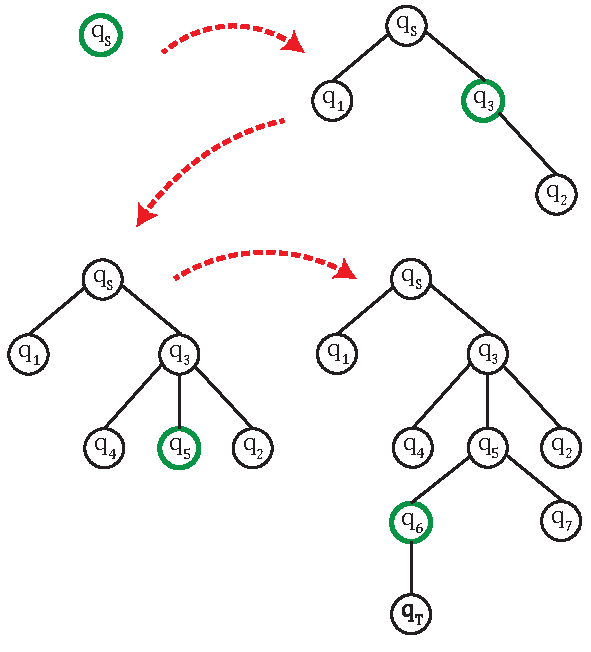
\includegraphics[width=300px]{images/path_database_build_process.pdf}
	\caption{A fa építésének folyamata}
	\label{fig:treeBuilding}
\end{figure}

\begin{explain}
A példában a $q_S$ pontot helyezzük először az adatbázisba, így az lesz a fa gyökere. Mivel ez az egyetlen pont, amit ki tudunk terjeszteni, ezt használjuk \emph{landmark-nak}. Ennél a kiterjesztésnél kerülnek a fába a $q_1, q_2, q_3$ pontok. Ezek közül $q_1$ és $q_2$ a két generált RC, és $q_3$ az egyikhez vezető úton egy irányváltási pont. A költségszámítás alapján a következő legkedvezőbb pont $q_3$, tehát kiterjesztjük, így megkapjuk a két RC-t: $q_4$-et és $q_5$-öt. Ez alkalommal nem kellett irányt váltani a \emph{waypoint-hoz} vezető úton, így nem keletkezik köztes pont. A következő lépésben a $q_5$ RC-t használjuk, hogy újabb \emph{waypoint-okat} generáljunk, ezek lesznek $q_6$ és $q_7$. Ebben a lépésben találjuk meg a $q_T$ célpontot is a $q_6$ RC-ből kiindulva, ezért $q_6$ egyetlen gyereke $q_T$ lesz.
\end{explain}

Ezen kívül a {\fontfamily{cmtt}\selectfont CPathDatabase} osztály feladata még az uniform méretű \emph{Motion Primitive-ek-en} kívüli dinamikus hosszúságú mozdulatok hosszú távú tárolása is. Erre azért van szükség, mert az útvonaltervező eredeti implementációjában ezek minden tervezés után törlődtek. Mivel a \emph{Waypoint Modul} használatával legjobb esetben is 2 tervezés történik, szükség van ezek mentésére.
\clearpage

A tárolást megvalósító C++ implementáció a {\fontfamily{cmtt}\selectfont CConnectingPrimitiveContainer} osztály. Ilyen típusú objektumokat tárol a {\fontfamily{cmtt}\selectfont CPathDatabase} osztály egy, az előzőnél egyszerűbb \emph{map}-ban. \\

\lstset{caption={A {\fontfamily{cmtt}\selectfont CConnectingPrimitiveContainer} osztály}, label=src:connPrimiContainer}
\begin{lstlisting}[language={C++}]
class CConnectingPrimitiveContainer
{
public:
    CConnectingPrimitiveContainer() = default;

    CConnectingPrimitiveContainer(const CConnectingPrimitiveContainer& f_other);

    void addPrimitive(const CMotionPrimitiveBase* f_primitive);

    vfc::TFixedVector<const CMotionPrimitiveBase*, 5> getPrimitivePointers() const;

private:
    vfc::TFixedVector<CCircleMotionPrimitive, 4>      m_circlePrimitives;
    vfc::TFixedVector<CLineMotionPrimitive, 1>        m_linePrimitives;
    vfc::TFixedVector<const CMotionPrimitiveBase*, 5> m_primitivePointers;
};
\end{lstlisting}

Mivel a \emph{Motion Primitive-ek} absztrakt ősosztály segítségével vannak implementálva, ezért nem lehet őket direkt példányosítani. A belőlük leszármazó {\fontfamily{cmtt}\selectfont CLineMotionPrimitive} és {\fontfamily{cmtt}\selectfont CCircleMotionPrimitive} objektumokat példányosítjuk, és a rájuk mutató \emph{pointer-eket} adjuk vissza lekérdezés esetén. Azt, hogy egy \emph{Motion Primitive} melyik kategóriába esik, a primitív $\delta$ paramétere alapján tudjuk eldönteni, hiszen az egyenes irányú mozgáshoz nem szükséges kormányszöget változtatni. Ezen felül szükséges még felülírni az osztályhoz tartozó \emph{copy constructor-t}, mert másolás esetén a régi objektum \emph{pointer-eit} fogja tárolni az eredmény, ami érvénytelen hivatkozásokat eredményez.
\clearpage

\begin{note}
Mind a dinamikus hosszúságú primitívek tárolása, és a leszármazott osztályok példányosítása is azért szükséges, mert a projekt keretein belül nem használható dinamikus memória. Ellenkező esetben a {\fontfamily{cmtt}\selectfont new} kulcsszó segítségével könnyebben kezelhető lenne a \emph{Motion Primitive-ek} tárolása. Ilyenkor viszont figyelni kell, hogy a {\fontfamily{cmtt}\selectfont delete}-t használjuk a foglalt memóriának a felszabadítására. A C++ nyelvben több lehetőség is lenne ennek automatizálására, az itt megfelelő módszer az {\fontfamily{cmtt}\selectfont std::shared\_ptr} lenne, amely automatikusan törlődik, ha az összes őt birtokló objektum is törlődik. \cite{shared_ptr}
\end{note}